\documentclass{article}
\usepackage{amsmath}
\usepackage{amssymb}
\usepackage[spanish]{babel}
\usepackage{color}
\usepackage{colortbl}
\usepackage{float}
\usepackage[T1]{fontenc}
\usepackage[rmargin=3cm,lmargin=3cm,tmargin=3cm,bmargin=4cm]{geometry}
\usepackage[utf8]{inputenc}
\usepackage{latexsym}
\usepackage{multirow}
\usepackage[spanish]{syllogism}
\usepackage{tikz}
\usepackage{tikz-qtree}
\usepackage{upgreek}

\clubpenalty=10000
\widowpenalty=10000

\begin{document}

\title{Ayudantía Unidad 1: Lógica (parte 3)}
\author{Teoría de la Computación 2-2025}
\date{}

\maketitle

\section{Lógica de primer orden: UMG}

Determine, si es posible, el unificador de máxima generalidad, indicando cada uno de los pasos para su obtención:

\subsection{UMG 1}

$$E = f(x_{1},\ x_{3},\ x_{2})$$
$$F = f(g(x_{2}),\ j(x_{4}),\ h(x_{3}, a))$$

\textbf{Solución:}\\ Aplicando el algoritmo de Robinson:

\begin{itemize}
  \item $k = 0$
  \begin{align*}
    &\sigma_{0} = \{\}\\
    &E_{0} = \sigma_{0}(E) = f(x_{1},\ x_{3},\ x_{2})\\
    &F_{0} = \sigma_{0}(F) = f(g(x_{2}),\ j(x_{4}),\ h(x_{3}, a))
  \end{align*}


  \item $k = 1$: par de discordancia $(x_{1},\ g(x_{2}))$
  \begin{align*}
    &\sigma_{1} = \{x_{1} / g(x_{2})\}\\
    &E_{1} = \sigma_{1}(E_{0}) = f(g(x_{2}),\ x_{3},\ x_{2})\\
    &F_{1} = \sigma_{1}(F_{0}) = f(g(x_{2}),\ j(x_{4}),\ h(x_{3}, a))
  \end{align*}


  \item $k = 2$: par de discordancia $(x_{3},\ j(x_{4}))$
  \begin{align*}
    &\sigma_{2} = \{x_{3}/j(x_{4})\}\\
    &E_{2} = \sigma_{2}(E_{1}) = f(g(x_{2}),\ j(x_{4}),\ x_{2})\\
    &F_{2} = \sigma_{2}(F_{1}) = f(g(x_{2}),\ j(x_{4}),\ h(j(x_{4}), a))
  \end{align*}


  \item $k = 3$: par de discordancia $(x_{2},\ h(j(x_{4}), a))$
  \begin{align*}
    &\sigma_{3} = \{x_{2}/h(j(x_{4}, a))\}\\
    &E_{3} = \sigma_{3}(E_{2}) = f(g(h(j(x_{4}, a))),\ j(x_{4}),\ h(j(x_{4}, a)))\\
    &F_{3} = \sigma_{3}(F_{2}) = f(g(h(j(x_{4}, a))),\ j(x_{4}),\ h(j(x_{4}), a))
  \end{align*}
\end{itemize}

Dado que $E_{3} = F_{3}$, logramos unificar las expresiones $E$ y $F$ originales
con el UMG:
$$\sigma = \sigma_{3} \circ \sigma_{2} \circ \sigma_{1} = \{x_{1} / g(h(j(x_{4}, a))),\ x_{3}/j(x_{4}),\ x_{2}/h(j(x_{4}, a))\}$$


\subsection{UMG 2}
$$E = q(f(a),\ g(b, Y),\ m(X, f(Z)))$$
$$F = q(X,\ g(b, c),\ m(f(a), Z))$$

\textbf{Solución:}\\ Aplicando el algoritmo de Robinson:

\begin{itemize}
  \item $k = 0$
  \begin{align*}
    &\sigma_{0} = \{\}\\
    &E_{0} = \sigma_{0}(E) = q(f(a),\ g(b, Y),\ m(X, f(Z)))\\
    &F_{0} = \sigma_{0}(F) = q(X,\ g(b, c),\ m(f(a), Z))
  \end{align*}

  \item $k = 1$: par de discordancia $(f(a),\ X)$
  \begin{align*}
    &\sigma_{1} = \{X/f(a)\}\\
    &E_{1} = \sigma_{1}(E_{0}) = q(f(a),\ g(b, Y),\ m(f(a), f(Z)))\\
    &F_{1} = \sigma_{1}(F_{0}) = q(f(a),\ g(b, c),\ m(f(a), Z))
  \end{align*}

  \item $k = 2$: par de discordancia $(g(b, Y),\ g(b, c))$
  \begin{align*}
    &\sigma_{2} = \{Y/c\}\\
    &E_{2} = \sigma_{2}(E_{1}) = q(f(a),\ g(b, c),\ m(f(a), f(Z)))\\
    &F_{2} = \sigma_{2}(F_{1}) = q(f(a),\ g(b, c),\ m(f(a), Z))
  \end{align*}
\end{itemize}

Notemos que la única discordancia restante es el término $f(Z)$ en $E_{2}$ y la
variable $Z$ en $F_{2}$. Sin embargo, como el término contiene la variable, significa que hay un \textit{occur check} y por lo tanto no es posible encontrar un unificador para las expresiones $E$ y $F$ originales.


\newpage


\section{Lógica de primer orden: resolución}

\subsection{Resolución 1}
Demuestre usando resolución la validez de:
$$\forall x [P(x) \rightarrow Q(x)] \vDash \forall y [\neg Q(y) \rightarrow \neg P(y)]$$

\textbf{Solución:}

El primer paso es transformar $\Sigma \cup \{\neg \upvarphi\}$ a forma normal de Skolem:

\begin{itemize}

  \item{\makebox[8cm][l]{$\forall x [P(x) \rightarrow Q(x)] = \forall x [\underbrace{\neg P(x) \vee Q(x)}_{C_{1}}]$}
        (premisa)}

  \item{\makebox[8cm][l]{$\neg \forall y [\neg Q(y) \rightarrow \neg P(y)] = \neg \forall y [Q(y) \vee \neg P(y)]$}
        (negación de la consecuencia)}

        {\makebox[8cm][l]{$\phantom{\neg \forall y [\neg Q(y) \rightarrow \neg P(y)]} = \exists y \neg [Q(y) \vee \neg P(y)]$}
        ($\neg \forall y \upvarphi \Leftrightarrow \exists y \neg \upvarphi$)}

        {\makebox[8cm][l]{$\phantom{\neg \forall y [\neg Q(y) \rightarrow \neg P(y)]} = \exists y [\neg Q(y) \land P(y)]$}
        (De Morgan)}

        {\makebox[8cm][l]{$\phantom{\neg \forall y [\neg Q(y) \rightarrow \neg P(y)]} = \underbrace{\neg Q(C)}_{C_{2}} \land \underbrace{P(C)}_{C_{3}}$}
        (skolemización, $C$ es una constante)}
\end{itemize}

Finalmente aplicamos la regla de resolución, unificando las expresiones cuando sea necesario:

\begin{figure}[H]
  \centering
  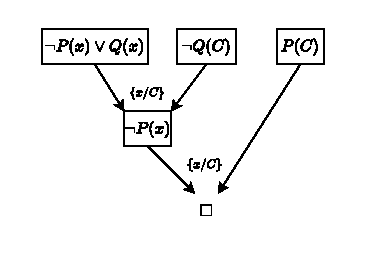
\includegraphics[width=.5\textwidth]{resolucion_lpo_01.pdf}
\end{figure}


\newpage


\subsection{Resolución 2}
Exprese los siguientes enunciados como fórmulas de lógica de primer orden:
\begin{enumerate}
  \item Todo dragón es feliz si todos sus hijos pueden volar.
  \item Los dragones verdes pueden volar.
  \item Un dragón es verde si es hijo de al menos un dragón verde.
\end{enumerate}

Demuestre usando resolución que la conjunción de estos 3 enunciados implica lo
siguiente: todos los dragones verdes son felices.\\ \\


\textbf{Solución:}\\
Definiremos los siguientes predicados:

\begin{itemize}
  \item $H(x)$: $x$ es feliz
  \item $F(x)$: $x$ puede volar
  \item $G(x)$: $x$ es verde
  \item $C(y, x)$: $y$ es hijo de $x$
\end{itemize}

Así, las premisas $F_{1}, F_{2}, F_{3}$ y la conclusión $F_{4}$ se expresarán
como:

\begin{enumerate}
  \item $F_{1} = \forall x [\forall y (C(y, x) \rightarrow F(y)) \rightarrow H(x)]$
  \item $F_{2} = \forall x [G(x) \rightarrow F(x)]$
  \item $F_{3} = \forall x [\exists y (C(x,y) \land G(y)) \rightarrow G(x)]$
  \item $F_{4} = \forall x [G(x) \rightarrow H(x)]$
\end{enumerate}

Ahora debemos transformar estas expresiones a forma normal de Skolem:

\begin{itemize}

  \item{\makebox[10cm][l]{$F_{1} = \forall x [\forall y (C(y, x) \rightarrow F(y)) \rightarrow H(x)]$}
    (premisa 1)}

        {\makebox[10cm][l]{$\phantom{F_{1}} = \forall x [\forall y (\neg C(y, x) \vee F(y)) \rightarrow H(x)]$}
        (eliminación del condicional)}

        {\makebox[10cm][l]{$\phantom{F_{1}} = \forall x [\neg \forall y (\neg C(y, x) \vee F(y)) \vee H(x)]$}
        (eliminación del condicional)}

        {\makebox[10cm][l]{$\phantom{F_{1}} = \forall x [\exists y \neg(\neg C(y, x) \vee F(y)) \vee H(x)]$}
        ($\neg \forall y \upvarphi \Leftrightarrow \exists y \neg \upvarphi$)}

        {\makebox[10cm][l]{$\phantom{F_{1}} = \forall x [\exists y (C(y, x) \land \neg F(y)) \vee H(x)]$}
        (De Morgan)}

        {\makebox[10cm][l]{$\phantom{F_{1}} = \forall x \exists y [(C(y, x) \land \neg F(y)) \vee H(x)]$}
        (exteriorizar cuantificador)}

        {\makebox[10cm][l]{$\phantom{F_{1}} = \forall x \exists y [(C(y, x) \vee H(x)) \land (\neg F(y) \vee H(x))]$}
        (distributividad)}

        {\makebox[10cm][l]{$\phantom{F_{1}} = \forall x [\underbrace{(C(f(x), x) \vee H(x))}_{C_{1}} \land \underbrace{(\neg F(f(x)) \vee H(x))}_{C_{2}}]$}
        (skolemización)}


  \item{\makebox[10cm][l]{$F_{2} = \forall x [G(x) \rightarrow F(x)]$} (premisa
        2)}

        {\makebox[10cm][l]{$\phantom{F_{2}} = \forall x [\underbrace{\neg G(x) \vee F(x)}_{C_{3}}]$}
        (eliminación del condicional)}


  \item{\makebox[9cm][l]{$F_{3} = \forall x [\exists y (C(x,y) \land G(y)) \rightarrow G(x)]$}
        (premisa 3)}

        {\makebox[9cm][l]{$\phantom{F_{3}} = \forall x [\neg \exists y (C(x,y) \land G(y)) \vee G(x)]$}
        (eliminación del condicional)}

        {\makebox[9cm][l]{$\phantom{F_{3}} = \forall x [\forall y \neg(C(x,y) \land G(y)) \vee G(x)]$}
        ($\neg \exists y \upvarphi \Leftrightarrow \forall y \neg \upvarphi$)}

        {\makebox[9cm][l]{$\phantom{F_{3}} = \forall x [\forall y (\neg C(x,y) \vee \neg G(y)) \vee G(x)]$}
        (De Morgan)}

        {\makebox[9cm][l]{$\phantom{F_{3}} = \forall x \forall y [\underbrace{\neg C(x,y) \vee \neg G(y) \vee G(x)}_{C_{4}}]$}
        (extereorizar cuantificador)}


  \item{\makebox[9cm][l]{$\neg F_{4} = \neg \forall x [G(x) \rightarrow H(x)]$}
        (negación de la consecuencia)}

        {\makebox[9cm][l]{$\phantom{\neg F_{4}} = \neg \forall x [\neg G(x) \vee H(x)]$}
        (eliminación del condicional)}

        {\makebox[9cm][l]{$\phantom{\neg F_{4}} = \exists x \neg [\neg G(x) \vee H(x)]$}
        ($\neg \forall x \upvarphi \Leftrightarrow \exists x \neg \upvarphi$)}

        {\makebox[9cm][l]{$\phantom{\neg F_{4}} = \exists x [G(x) \land \neg H(x)]$}
        (De Morgan)}

        {\makebox[9cm][l]{$\phantom{\neg F_{4}} = \underbrace{G(a)}_{C_{5}} \land \underbrace{\neg H(a)}_{C_{6}}$}
        (skolemización, $a$ es una constante)}
\end{itemize}

Para concluir, se debe aplicar la regla de resolución sobre el conjunto de cláusulas encontrado:

\begin{figure}[H]
  \centering
  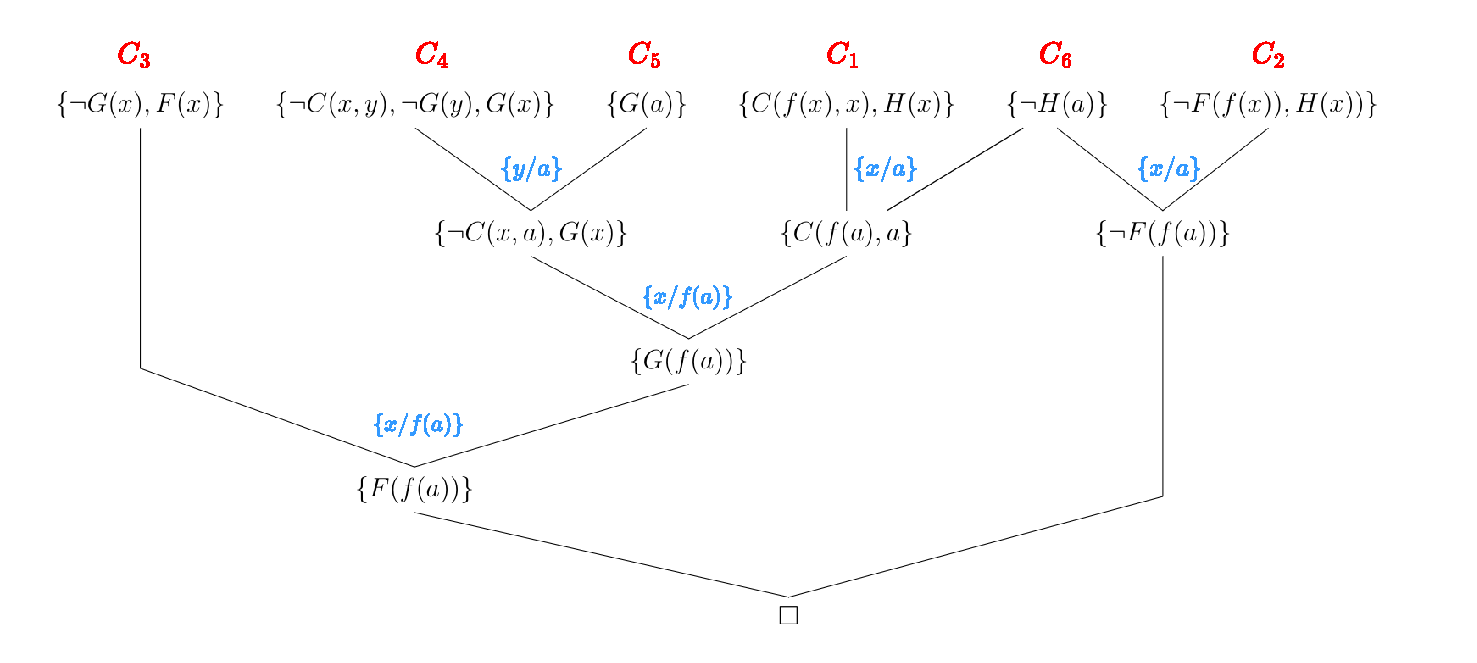
\includegraphics[width=.9\textwidth]{resolucion_lpo_02.pdf}
\end{figure}



\end{document}
